% !TEX root =  ../ReplyLetterMain.tex
\clearpage
\section*{Response to 1st Referee's Comments}
We would like to thank the Referee for his/her constructive comments, which have allowed us to considerably improve our paper. The main differences of the new version of the manuscript compared to the previous one can be found in Sections~2, 3 and 5. In addition, changes regarding the specific comments have been made throughout the text.
You may find below our response to the specific issues raised.

\begin{enumerate}
	\item With regards assumption of normality of random effects, joint models (JM) have been shown to be quite robust to random effects misspecification. More specifically, \citet*{rizopoulos2008shared,huang2009latent} have shown that unless the number of repeated measurements per person are extremely small, such misspecification only and trivially affects the standard errors. On the other hand in our dataset we have a mean of 8.7 measurements per person. 

	With regards to the assumption of normality of error term, we conducted residual diagnostics to check this assumption. The quantile-quantile (q-q) plot of subject specific residuals in Figure \ref{fig : qqplot_norm_t3} shows that a long tailed distribution for errors is more plausible than the normal distribution. Based on this result, we further fitted two JMs with t-distributed errors, with 4 and 3 degrees of freedom (df), respectively. We found that the model with t-distributed (df=3) errors satisfied the distributional assumptions the best (see Figure \ref{fig : qqplot_norm_t3}). 

	\begin{figure}[!htb]
	\centerline{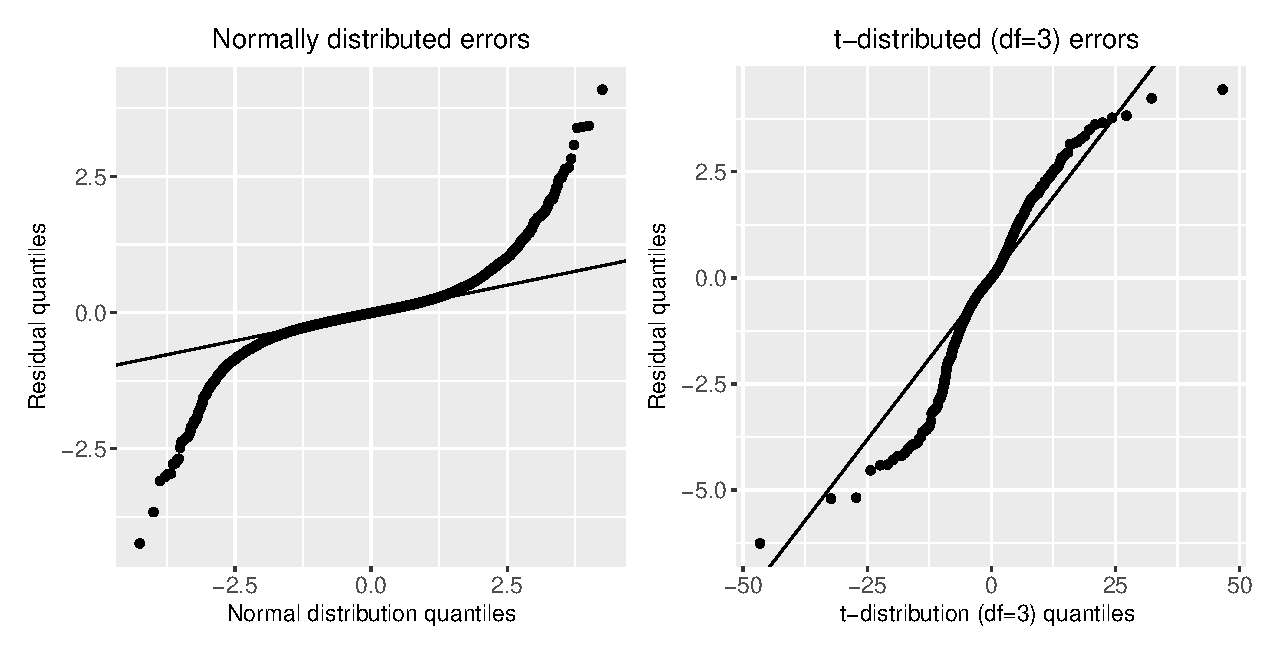
\includegraphics[width=\columnwidth]{images/model_fit/qqplot_norm_t3.eps}}
	\caption{Quantile-quantile plots of subject specific residuals obtained from joint models with assumption of normally distributed errors, and t-distributed (df=3) errors, fitted to the PRIAS data set.}
	\label{fig : qqplot_norm_t3}
	\end{figure}

	We then compared the model with assumption that errors are normally distributed and the model with assumption that errors are t-distributed. To this end, the fitted marginal $\log_2 \mbox{PSA}$ profile for a hypothetical patient with age 70 years using the two models is shown in Figure \ref{fig : marginal_fitted_psa_NormalVsT3}. We also compared the subject specific fitted $\log_2 \mbox{PSA}$ profiles for 9 randomly selected patients (each with more than 3 observations). A seed of 2017 (year of submission of the article) was used to sample these patients from the PRIAS dataset sorted by patient ID. Lastly, for the two models, Table \ref{tab : relative_risk_comparison} shows the association parameters. We can see that the association between the hazard of GR and slope of $\log_2 \mbox{PSA}$ is stronger in the model with t-distributed (df=3) errors. In light of the better fit of the model with t-distributed (df=3) errors, we have updated the parameters estimates in \ref{sec : param_estimates_jm_fit_prias} of the updated supplementary material.

	\begin{table}[!htb]
	\begin{center}
	\caption{Relative risk sub-model estimates for association parameters between hazard of GR and slope of $\log_2 \mbox{PSA}$ levels. Mean and 95\% credible interval (CI) are presented for fits obtained from joint model with assumption of normal distributed errors, and t-distributed (df=3) errors.}
	\label{tab : relative_risk_comparison}
	\begin{tabular}{lrr}
	\Hline
	Error distribution                      & $\log_2 \mbox{PSA}$ association [95\% CI]   & Slope($\log_2 \mbox{PSA}$) association [95\% CI]\\ 
	\hline
	t-distribution (df=3)                  & -0.004 [-0.119, 0.117] & 2.888 [2.318, 3.452] \\
	Normal distribution                    & -0.049 [-0.172, 0.078] & 2.407 [1.791, 3.069] \\
	\hline
	\end{tabular}	
	\end{center}
	\end{table}

	\begin{figure}[!htb]
	\centerline{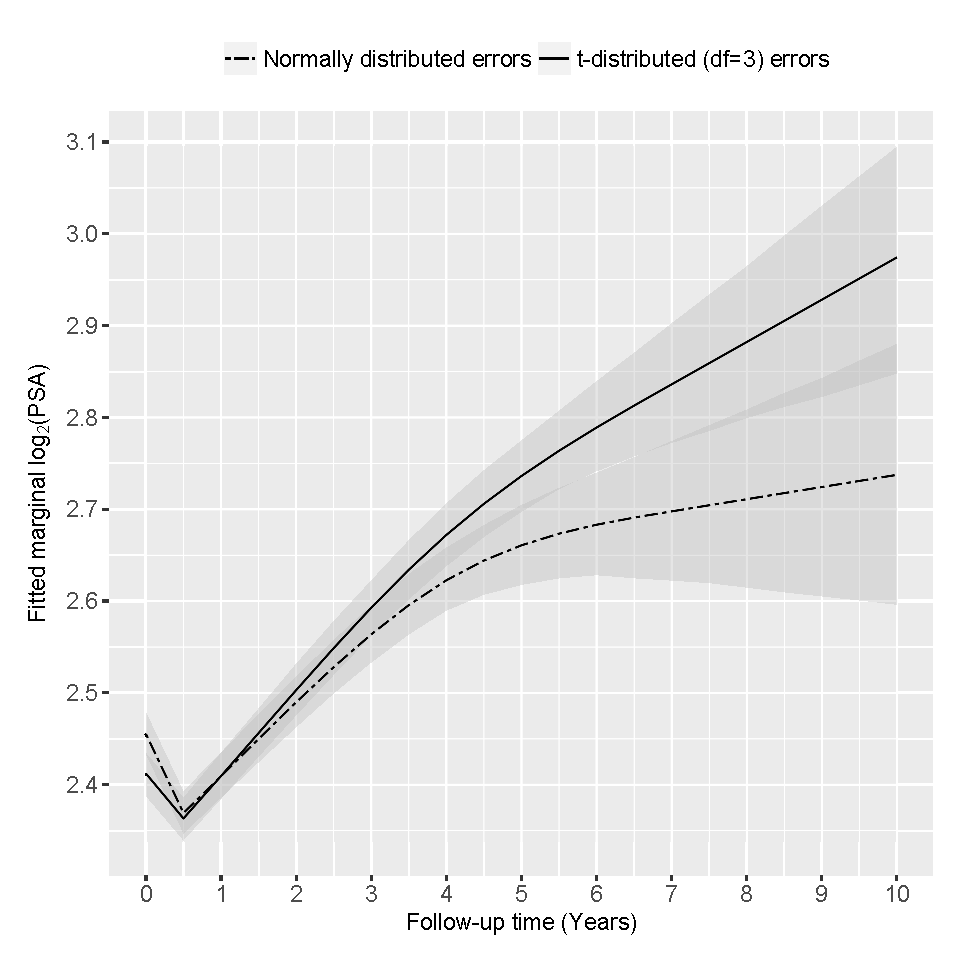
\includegraphics[width=0.75\columnwidth]{images/model_fit/marginal_fitted_psa_NormalVsT3.eps}}
	\caption{Fitted marginal 10 year $\log_2 \mbox{PSA}$ profile with 95\% credible interval (CI), for a hypothetical patient who was included in AS at the age of 70 years. Fits were obtained from joint models with assumption of normal distributed errors, and t-distributed (df=3) errors. The darker shaded region indicates the overlap in the two CI intervals, as well as demarcates the two sets of CIs.}
	\label{fig : marginal_fitted_psa_NormalVsT3}
	\end{figure}		
	
    \begin{figure}[!htb]
	\centerline{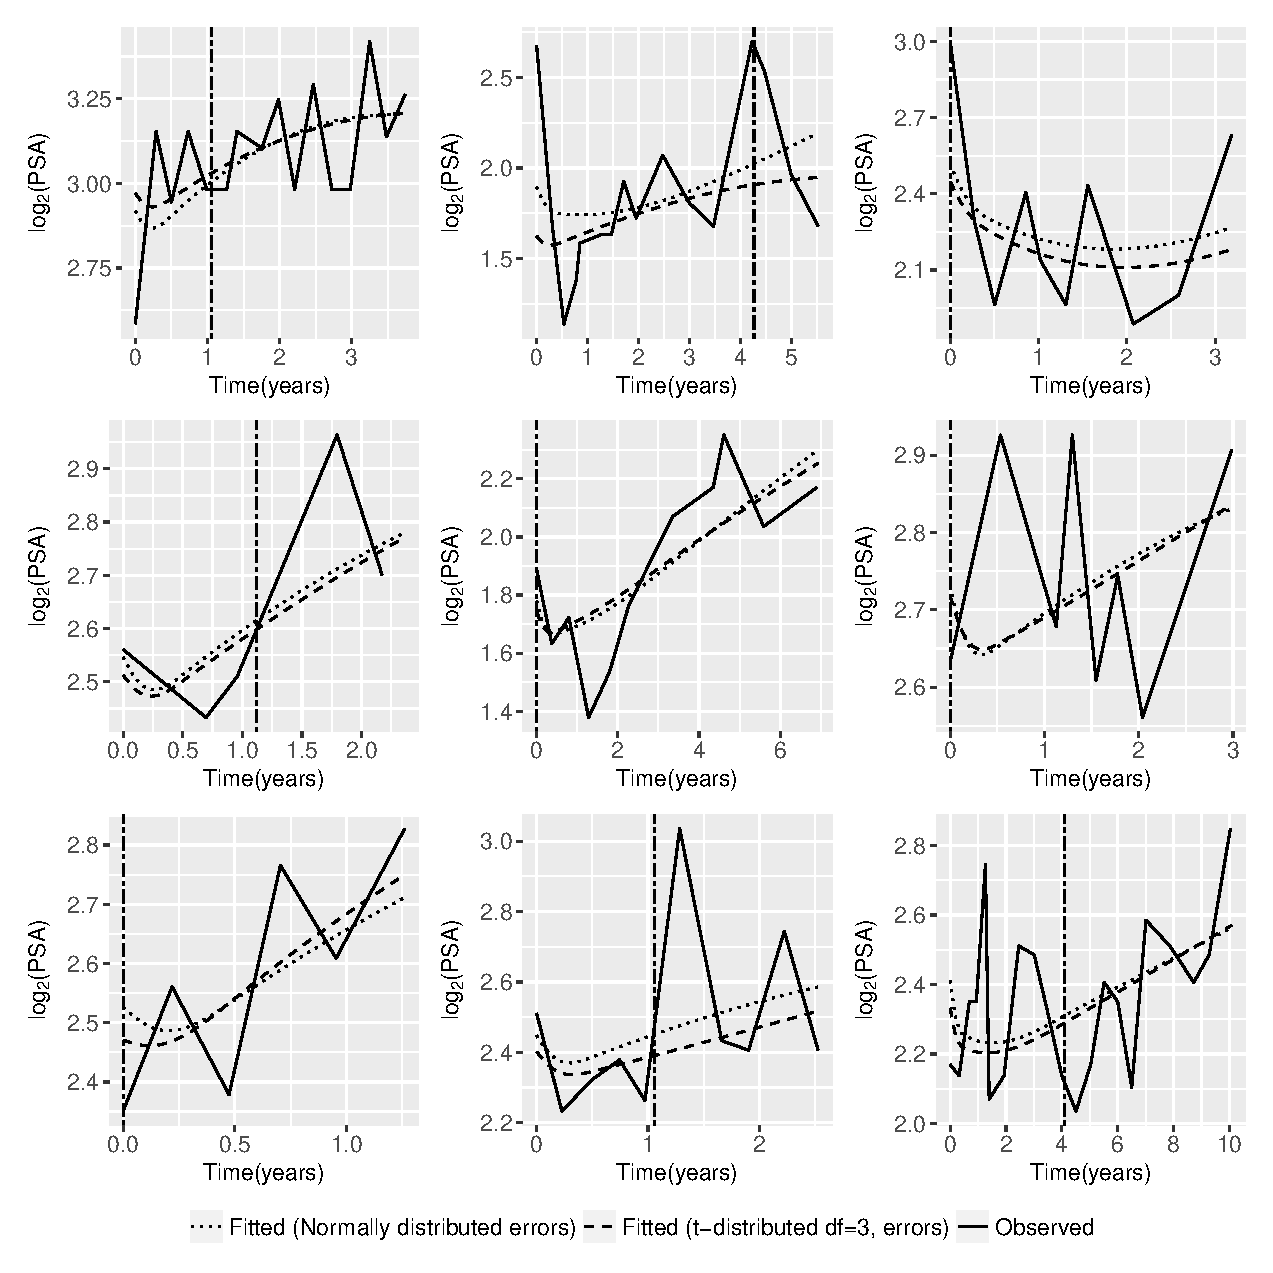
\includegraphics[width=\columnwidth]{images/model_fit/subject_fittedVsObserved_psa_norm_t3.eps}}
	\caption{Fitted versus observed $\log_2 \mbox{PSA}$ profiles for 9 randomly selected patients. Fits were obtained from joint models with assumption of normal distributed errors, and t-distributed (df=3) errors. The vertical line with a dot-dash pattern shows the time of the latest biopsy. The fitted profiles utilize information from both the observed PSA levels and time of latest biopsy.}
	\label{fig : subject_fittedVsObserved_psa_norm_t3}
	\end{figure}

	Since the slope association between $\log_2 \mbox{PSA}$ levels and hazard of Gleason reclassification (GR) in the model with t-distributed (df=3) has become stronger, we expect our schedules to become slightly more sensitive towards increase in $\log_2 \mbox{PSA}$ velocity. This however may also depend on the type of personalized schedule. For example, we compared the personalized schedule based on dynamic risk of GR using the two different models for the three demonstration patients, and observed trivial differences. This is however due to the fact that average risk (averaged over all time points) taken by dynamic risk of GR is not very high (5.3\%). However quantiles corresponding to 50\% risk (median time of GR) may differ by a bigger margin depending upon the profile of the patient (same for expected failure time). For example, we can see in Figure \ref{fig : demo_expfail_norm_t3} and Figure \ref{fig : variance_demo_patients} that the third demonstration patient has a consistent profile, with quite slow rise in PSA. Consequently the effect of the increased $\log_2 \mbox{PSA}$ slope association parameter does not affect the schedule much for this patient. Similar results are observed for the first demonstration patient when the PSA consistently remains low over nearly three years, starting at year two. Lastly, this can also be seen for the second demonstration patient wherein the schedules differ by a large margin when PSA rises very quickly. However the gap becomes slightly smaller after a negative biopsy indicating that GR is unlikely in near future. Thus we expect that the sensitivity of the schedule based on expected failure time is within acceptable boundaries for slowly progressing (low risk) patients.

	\begin{figure}[!htb]
	\centerline{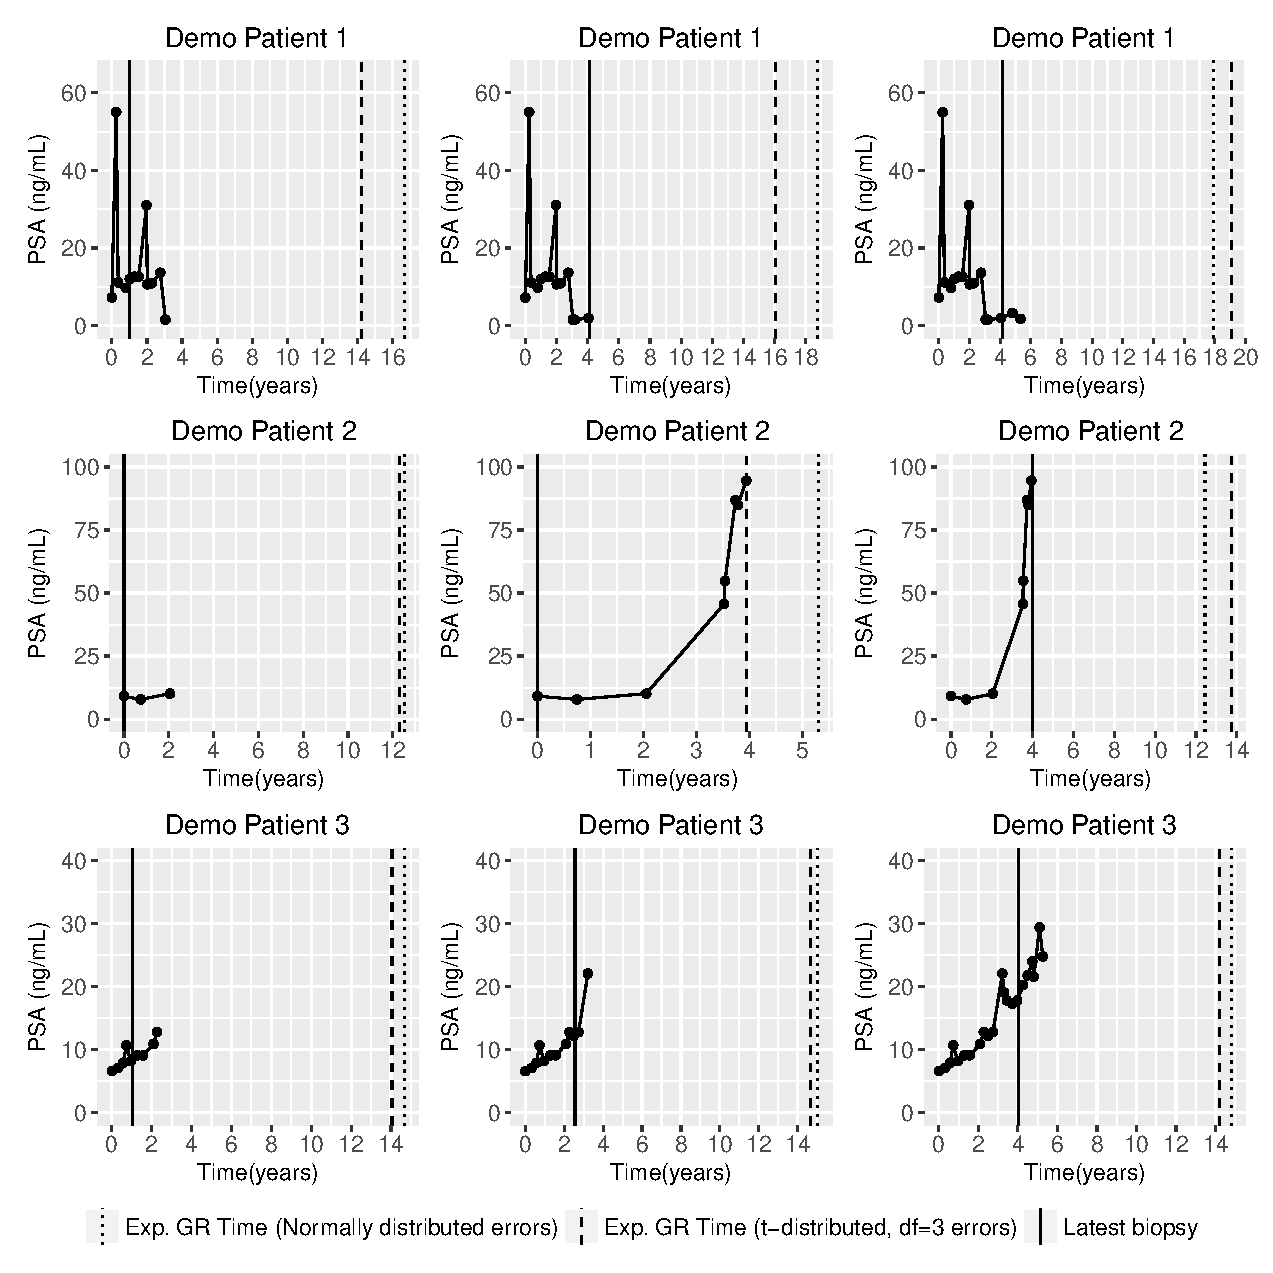
\includegraphics[width=\columnwidth]{images/model_fit/demo_expfail_norm_t3.eps}}
	\caption{Dynamic expected failure time for the three demonstration patients at three different follow-up times, using joint models with assumption of normal distributed errors, and t-distributed (df=3) errors.}
	\label{fig : demo_expfail_norm_t3}
	\end{figure}

	\begin{figure}[!htb]
	\centerline{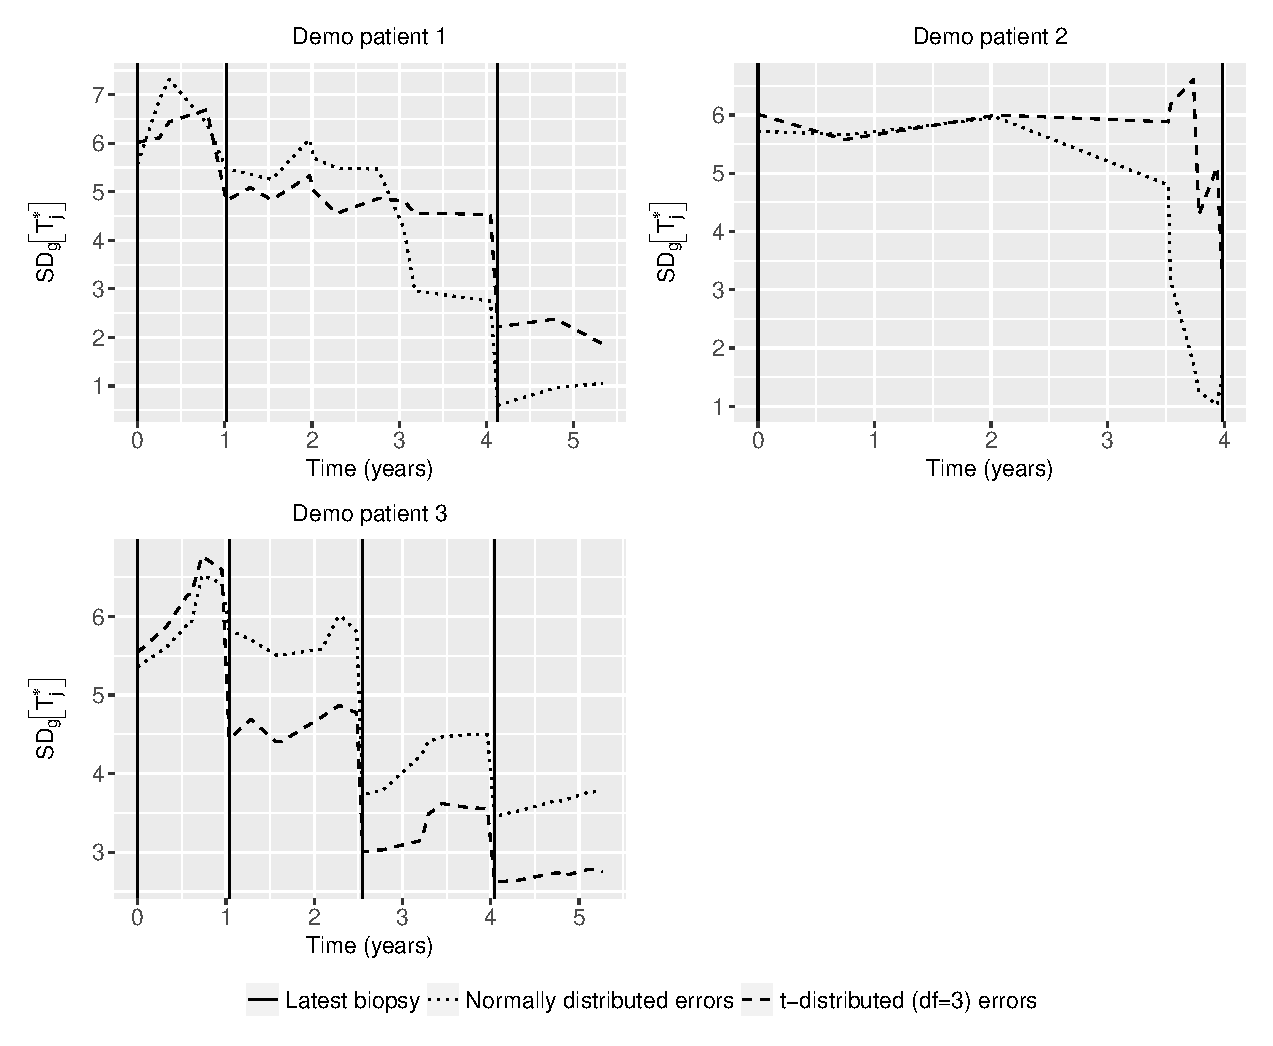
\includegraphics[width=\columnwidth]{images/model_fit/variance_demo_patients_norm_t3.eps}}
	\caption{Dynamic variance of the posterior predictive distribution of event time for the three demonstration patients at three different follow-up times, using joint models with assumption of normal distributed errors, and t-distributed (df=3) errors.}
	\label{fig : variance_demo_patients_norm_t3}
	\end{figure}

	\item The three patients were chosen on the basis of specific characteristics of their data. This is because we wanted to demonstrate three main features of the personalized schedules. For example, the first demonstration patient had many repeat biopsies, and thus via his profile we show how the variance of posterior predictive distribution of GR time decreases with each biopsy. Via the second demonstration patient we show how the schedules change with changes in PSA alone (no repeat biopsies). Whereas, via the third demonstration patient we show how the schedules work when information from PSA and repeat biopsies is not in concordance with each other. We would like to also mention that it is not the case that we conducted an exhaustive search to purposefully select only these three patients. 

	With regards to conducting cross-validation on real data, and to compare the true GR time of PRIAS patients who obtained GR, with the time proposed by personalized schedules, this is not possible for the following reason. For patients in PRIAS we only know the interval $l_i < T^*_i \leq r_i$ in which GR occurred and not the true GR time $T^*_i$. On top of that this is known only for 707 out of 5267 patients, and the rest are right censored. That is, in either case we cannot calculate the offset $T^S_i - T^*_i$ of our schedule, where $T^S_i > T^*_i$ is the time of the last biopsy at which GR is detected. The simulation study is our attempt to obviate this problem, because there we know the true event time $T^*_i$ for each of the patients. 

	\item We assume that there are three equal sized subgroups $G_1$, $G_2$ and $G_3$ of patients in the population, differing in the baseline hazard of GR. This was done because we wanted to test the performance of different schedules for a population with a mixture of patients, namely those with faster progressing PCa, as well as those with slowly progressing PCa. As advised by the referee this can be modeled using a stratified modeling approach. In the current case, this corresponds to the use of latent class JMs \citep{proust2014joint}. However this approach requires either knowing the number of subgroups in advance, which is unrealistic, or fitting multiple models to detect the correct number of subgroups. The latter would have been out of the scope of our paper. The alternative that we used was based on the fact that the baseline hazard in the simulated population corresponds to a mixture Weibull density \citep{razali2013mixture}. We model the log baseline hazard flexibly using P-splines. The mean of the fitted log baseline hazard between 0.1 years and 8 years (mean third quartile in the simulated progression times is 6.15 years), and 95\% confidence interval obtained from the 500 simulations is shown in Figure \ref{fig : fitted_baseline_hazard} below. It can be seen that the fit is quite close to the theoretical baseline hazard. We have added this figure and the corresponding summary in Section [section nr] of Supplementary material.

	\begin{figure}[!htb]
	\centerline{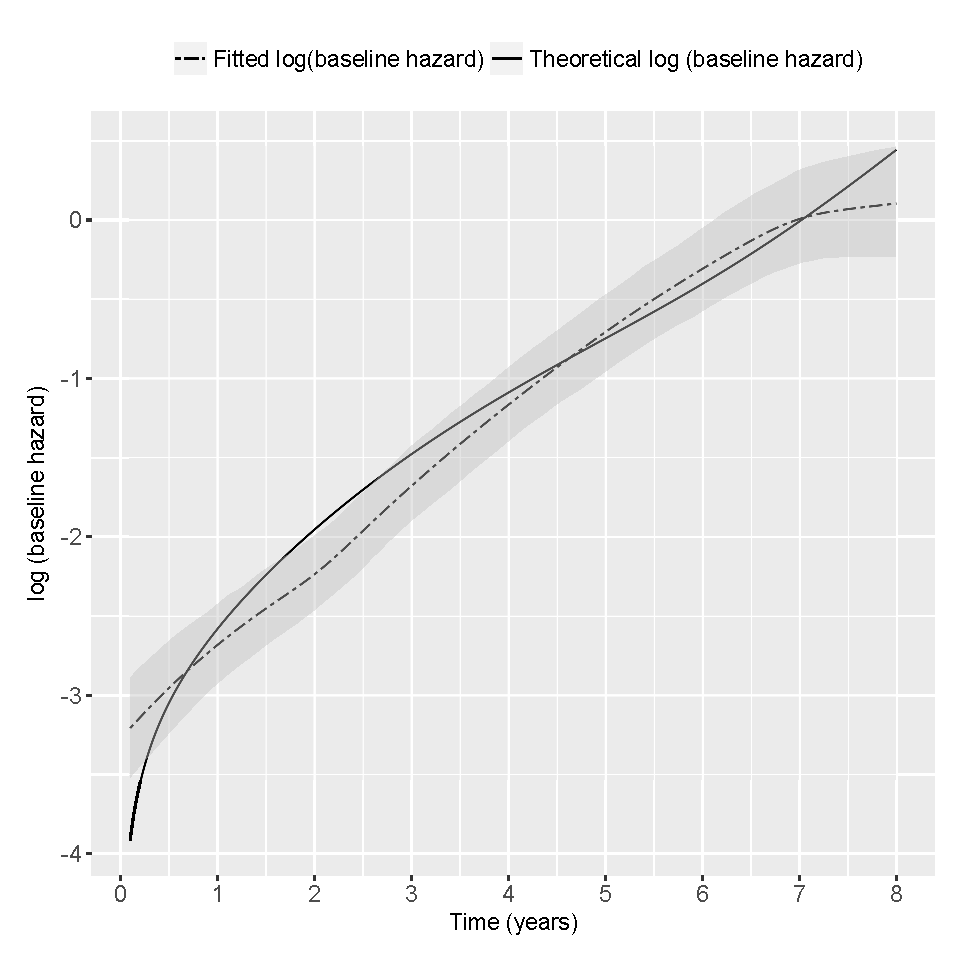
\includegraphics[width=0.75\columnwidth]{images/sim_study/baseline_hazard.eps}}
	\caption{Theoretical log baseline hazard of the simulated population versus mean of the fitted log baseline hazard. The 95\% confidence interval for the fitted log baseline hazard is obtained from the 500 simulations.}
	\label{fig : fitted_baseline_hazard}
	\end{figure}
	\item As noted by the referee, indeed PRIAS switches to the annual schedule if a patient's PSA doubling time (PSA-DT), measured as the inverse of the slope of the regression line through the base two logarithm of PSA values, is less than 10 years. In this regard, the joint model allows the schedule to depend upon the observed PSA values (e.g., via PSA-DT). This is because the parameters are estimated using a full likelihood approach \citep{tsiatis2004joint}. To show this, consider the following full general specification of the JM that we use. Let $\boldsymbol{y}_i$ denote the $n_i \times 1$ vector of PSA measurements for the $i$-th patient, and $l_i, r_i$ denote the two time points of the interval in which GR occurs for the $i$-th patient. In addition let $T_i^S$ and $\mathcal{V}_i$ denote the schedule of biopsies and schedule of PSA measurements, respectively. Under the assumption that both of these schedules may depend upon only the observed $\boldsymbol{y}_i$, the joint likelihood of all four processes is given by:

	\begin{equation}
	\label{eq : decomposition_likelihood}
	p(\boldsymbol{y}_i, l_i, r_i, T_i^S, \mathcal{V}_i \mid \boldsymbol{\theta}, \boldsymbol{\psi}) = p(\boldsymbol{y}_i, l_i, r_i \mid \theta) \times p(T_i^S, \mathcal{V}_i \mid \boldsymbol{y}_i, \boldsymbol{\psi})
	\end{equation}

	From this decomposition we can see that even if the processes $T_i^S$ and $\mathcal{V}_i$ may be determined from $\boldsymbol{y}_i$, if we are interested in the parameters $\boldsymbol{\theta}$ of the joint distribution of longitudinal and event outcome, we can maximize the likelihood based on the first term and ignore the second term. In other words, the second term will not carry information for $\boldsymbol{\theta}$.

	In order to demonstrate this we simulated a dataset with 750 patients. The true event times $T^*_i$ for these patients were generated using parameters from a joint model fitted to the PRIAS dataset. However this joint model did not include association between velocity of log PSA values and hazard of GR. That is, the hazard of GR $h_i(t)$ at any time $t$ depends only on the underlying log PSA value $m_i(t)$ at that time. Furthermore, for these patients we used the schedule of PRIAS to generate the interval $l_i \leq T^*_i \leq r_i$ in which GR is detected. Thus the observed data for $i$-th patient is $\{\boldsymbol{y}_i, l_i, r_i\}$. Our aim is to show that if there is no association between $h_i(t)$ and velocity of log PSA value $m'_i(t)$, then even though the biopsy schedule depends on PSA-DT (which is a crude measure of PSA velocity), a JM fitted with both value and velocity associations will have an insignificant velocity association. In the fitted JM we found the value association (95\% credible interval in brackets) to be 0.182 [0.090, 0.274], and the velocity association to be -0.001 [-0.295, 0.254]. That is even though the schedule of biopsies depended upon observed PSA values it did not lead to a spurious association. 

	With regards to the second question about the use of right censoring in the simulation study instead of interval censored data, this cannot lead to any differences in results. The reason is that we use a full likelihood approach as described in Section \ref{sec : jm_framework} of the original manuscript. Parameter estimation using full likelihood approaches always gives consistent and asymptotically unbiased results \citep{gentleman1994maximum}.

	\item The two sets of AUC's were mistakenly swapped while creating the table and hence the counterintuitive results. We have corrected this mistake, and in addition as advised by the referee, we have also reported the confidence interval. To obtain the 95\% confidence interval, we used 15 bootstrapped datasets of patients from the training dataset utilized in this paper. We calculate the AUC at year one, year two and year three of follow-up in AS. The time window for which the AUC is calculated is one year. The resulting estimates are presented in Table \ref{tab : AUC_reply_letter} below, as well as added in Supplementary material (\ref{tab : AUC}).

	\begin{table}[!htb]
	\begin{center}
	\caption{Area under the receiver operating characteristic curves, and 95\% confidence interval in brackets, obtained using 15 bootstrapped datasets.}
	\label{tab : AUC_reply_letter}
	\begin{tabular}{rrr}
\Hline
Year                      & $\log_2 \mbox{PSA}$ value and velocity association & $\log_2 \mbox{PSA}$ value association\\ 
\hline
1 & 0.613 [0.582, 0.632] & 0.595 [0.565, 0.618]\\
2 & 0.648 [0.608, 0.685] & 0.609 [0.568, 0.654]\\
3 & 0.593 [0.560, 0.638] & 0.590 [0.536, 0.628]\\
\hline
	\end{tabular}	
	\end{center}
	\end{table}

	\item We thank the referee for pointing out these errors. We have fixed these in the updated manuscript.

\end{enumerate}

